\documentclass[twoside]{article}
\usepackage{../../estilo-ejercicios}
\newcommand{\colapso}{{\searrow\!\!\!\!\searrow}}
%--------------------------------------------------------
\begin{document}

\title{Ejercicios de Teoría Geométrica de Grupos}
\author{Javier Aguilar Martín}
\maketitle

\section{Grupos finitamente generados como espacios métricos}

\begin{ejercicio}{1.1}
Dibujar los grafos de Cayley de:
\begin{enumerate}
\item $D_n=\gene{a,b\mid a^n=b^2=1,aba=b}$.
\item $D_\infty=\gene{a,b\mid b^2=1,aba=b}$.
\item Icosahedro: $\gene{a,b,c\mid a^2=b^2=c^2=(ab)^3=(ca)^5=(bc)^2=1}$.
\end{enumerate}

\end{ejercicio}
\begin{solucion}
\begin{enumerate}
\item Este es $D_4$, los demás similares pero con más lados. 
\begin{figure}[h!]
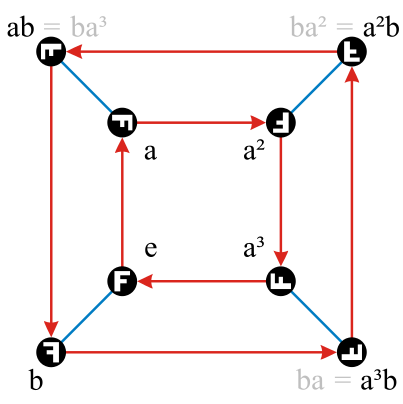
\includegraphics[scale=0.5]{Dih4}
\end{figure}
\item Está en los apuntes
\end{enumerate}
\end{solucion}

\newpage

\begin{ejercicio}{1.2}
Supongamos que $N\trianglelefteq G$ es finito y $G/N$ es finitamente generado. Entonces $G$ es quasi-isométrico a $G/N$. 
\end{ejercicio}
\begin{solucion}
Por ser $N$ finito y $G/N$ finitamente generado, $N$ tiene índice finito, de donde se deduce el resultado. 

\end{solucion}




\newpage

\begin{ejercicio}{1.3}
En $\Z$ consideramos las métricas
\[
d(x,y)=|x-y|,\quad d'(x,y)=|x-y|+\log(|x-y|), d'(x,x)=0
\]
y sea $Id:(\Z,d)\to(\Z,d')$. Demostrar que
\begin{enumerate}[a)]
\item para todo $\lambda>1$ existe $c\geq 0$ tal que $Id$ es una $(\lambda,c)$-quasi-isometría,
\item no existe $c\geq 0$ tal que $Id$ es una $(1,c)$-quasi-isometría.
\end{enumerate}
\end{ejercicio}
\begin{solucion}

\end{solucion}

\newpage

\begin{ejercicio}{1.4}
Sea $T_d$ el árbol $d$-regular. Demostrar que $T_3$ es quasi-isométrico a $T_4$.
\end{ejercicio}
\begin{solucion}
EN EL ENUNCIADO HAY UN DIBUJO. NO SÉ SI ES IMPORTANTE EL NÚMERO DE VÉRTICES, INTENTARLO DE CUALQUIER FORMA. 
\end{solucion}

\newpage

\begin{ejercicio}{1.5}
$\Z$ no es quasi-isométrico a $\Z^2$.
\end{ejercicio}
\begin{solucion}
SE PUEDE HACER FÁCIL CON EL SIGUIENTE TEMA, PERO INTENTAR CON LO DE ESTE
\end{solucion}

\newpage

\section{Invariantes de quasi-isometría: crecimiento}

\begin{ejercicio}{2.1}
Probar que $\beta_{\Z^k}\sim n^k$.
\end{ejercicio}
\begin{solucion}

\end{solucion}

\newpage

\begin{ejercicio}{2.2}
Calcular el crecimiento de $\left\{\begin{pmatrix}
1 & x & z\\
0 & 1 & y\\
0 & 0 & 1
\end{pmatrix}\middle\vert x,y,z\in\Z\right\}$. Ayuda: $a=\begin{pmatrix}
1 & 1 & 0\\
0 & 1 & 0\\
0 & 0 & 1
\end{pmatrix}$ y $b=\begin{pmatrix}
1 & 0 & 0\\
0 & 1 & 1\\
0 & 0 & 1
\end{pmatrix}$ generan el grupo, pero es más fácil si se considera también $c=\begin{pmatrix}
1 & 0 & 1\\
0 & 1 & 0\\
0 & 0 & 1
\end{pmatrix}$ como generador. 
\end{ejercicio}
\begin{solucion}
\url{https://en.wikipedia.org/wiki/Heisenberg_group}\url{http://www.math.uchicago.edu/~may/VIGRE/VIGRE2009/REUPapers/Lim.pdf}
\end{solucion}

\newpage

\begin{ejercicio}{2.3}
Probar las siguientes afirmaciones:
\begin{enumerate}
\item $\beta_{(G,X)}(n+m)\leq \beta_{(G,X)}(n)\beta_{(G,X)}(m)$.
\item $w(G,X)=\limsup_{n\to \infty}\sqrt[n]{\beta(G,X)(n)}$ es un límite. 
\item $G$ es de crecimiento exponencial si y solo si $w(G,X)>1$.
\end{enumerate}
\end{ejercicio}
\begin{solucion}

\end{solucion}

\newpage

\begin{ejercicio}{2.4}
Un grupo finitamente generado es \textbf{promediable} si existe una sucesión $\{F_n\}_{n\in\N}$ de conjuntos finitos tal que $\lim_{n\to\infty}\frac{|\partial F_n|}{|F_n|}=0$, donde $\partial F_n=\{x\in G\mid x\notin F, d(x,F)=1\}$.

Probar que si el crecimiento de $G$ no es exponencial, entonces $G$ es promediable. 
\end{ejercicio}
\begin{solucion}

\end{solucion}

\newpage

\section{Invariantes de quasi-isometría: finales}

EN PRINCIPIO NO HAY EJERCICIOS, TAL VEZ PONER AQUÍ ALGUNO DE LOS EJEMPLOS QUE SE DEJA COMO EJERCICIO

\section{Grupos finitamente presentados}
\begin{ejercicio}{3.1}

Sea $G=\gene{x,y\mid xy^2=y^3x, yx^2=x^3y}$. Probar que $G$ es trivial.
\end{ejercicio}
\begin{solucion}
Multiplicando las relaciones obtenemos ·$yx^3y^2=y^3x^4y\Rightarrow x^3y=y^2x^4=(yx^2)^2=(x^3y)^2\Rightarrow x^3y=1$. Sustituyendo en la primera relación tenemos que $yx^2=1$, por lo que $y^{-1}=x^2=x^3$, de donde se deduce que $x=y=1$.
\end{solucion}

\newpage

\begin{ejercicio}{3.2}
$\Z^n$ tiene función de Dehn cuadrática. 
\end{ejercicio}
\begin{solucion}
\end{solucion}

\newpage

\section{Lenguas formales}

\begin{ejercicio}{4.1}
Describir la lengua asociada al autómata del tercer ejemplo que no he puesto en los apuntes DIBUJAR AUTÓMATA
\end{ejercicio}
\begin{solucion}

\end{solucion}


\end{document}
